\section{Research Symposium}

\subsection{What is XPGRS}
XJTLU Postgraduate Research Symposium, abbreviated as XPGRS or Symposium, is an event organized by the Graduate School. Every year, commonly December, all PhD students in the university are invited to present their research results or progress through posters or oral presentations. Each year's XPGRS is announced via email around October.

\subsection{Which event do I need to participate in?}

The official requirements are as follows:

\begin{itemize}
    \item Second-year PhD students need to give poster presentations
    \item Third-year PhD students need to give oral presentations
    \item Fourth-year or above PhD students will be invited to serve as session chairs
    \item Master's students in the dissertation stage are also welcome to participate
\end{itemize}

Based on past experiences, this translates to:

\begin{itemize}
    \item First-year students have nothing required, but can consider volunteering (an email will be sent for recruitment) or simply attend to observe and learn about seniors' work
    \item Second-year students must do a poster
    \item Third-year students must give an oral presentation and may consider being a chair
    \item Fourth-year or above students are free to choose
\end{itemize}

To determine which year you are in, use December 1st of the current year as the reference. This is straightforward for those who enrolled between March and September, but many students happen to enroll on December 1st. According to the 2022 information, these students are required to participate, meaning, for example, if you enrolled in December 2021, you need to do a poster in 2022.
% These students can choose whether to participate after one year. For example:
% \begin{itemize}
%     \item Student A enrolled in December 2020. In December 2021, he found he had too little to show and decided not to participate. Therefore, he must do a poster in December 2022, an oral presentation in December 2023, and is free in December 2024.
%     \item Student B enrolled in December 2020. In December 2021, she felt she could present something and wanted to improve her skills early, also as preparation for future academic conferences. So she participated in the poster session in December 2021, then had to give an oral presentation in December 2022, and is free in December 2023.
% \end{itemize}
%
Of course, since December entrants are special cases, policies may change, so it's best to email (or call) the Graduate School each year to inquire.

Theoretically, you can participate in both poster and oral sessions every year if you wish! You can even choose not to participate at all, but you need your supervisor's approval. Generally, unless there's a special reason, supervisors hope you can gain experience. If there is a valid reason, your supervisor can contact the Graduate School, and with their agreement, you can opt out. (I've heard of supervisors who think the symposium is useless and have their students never participate, and some who have students do both poster and oral presentations from the start...)

\begin{figure}[H]
    \caption{Poster session of the 2021 Symposium (CB G13W), before the official start}
    \centering
    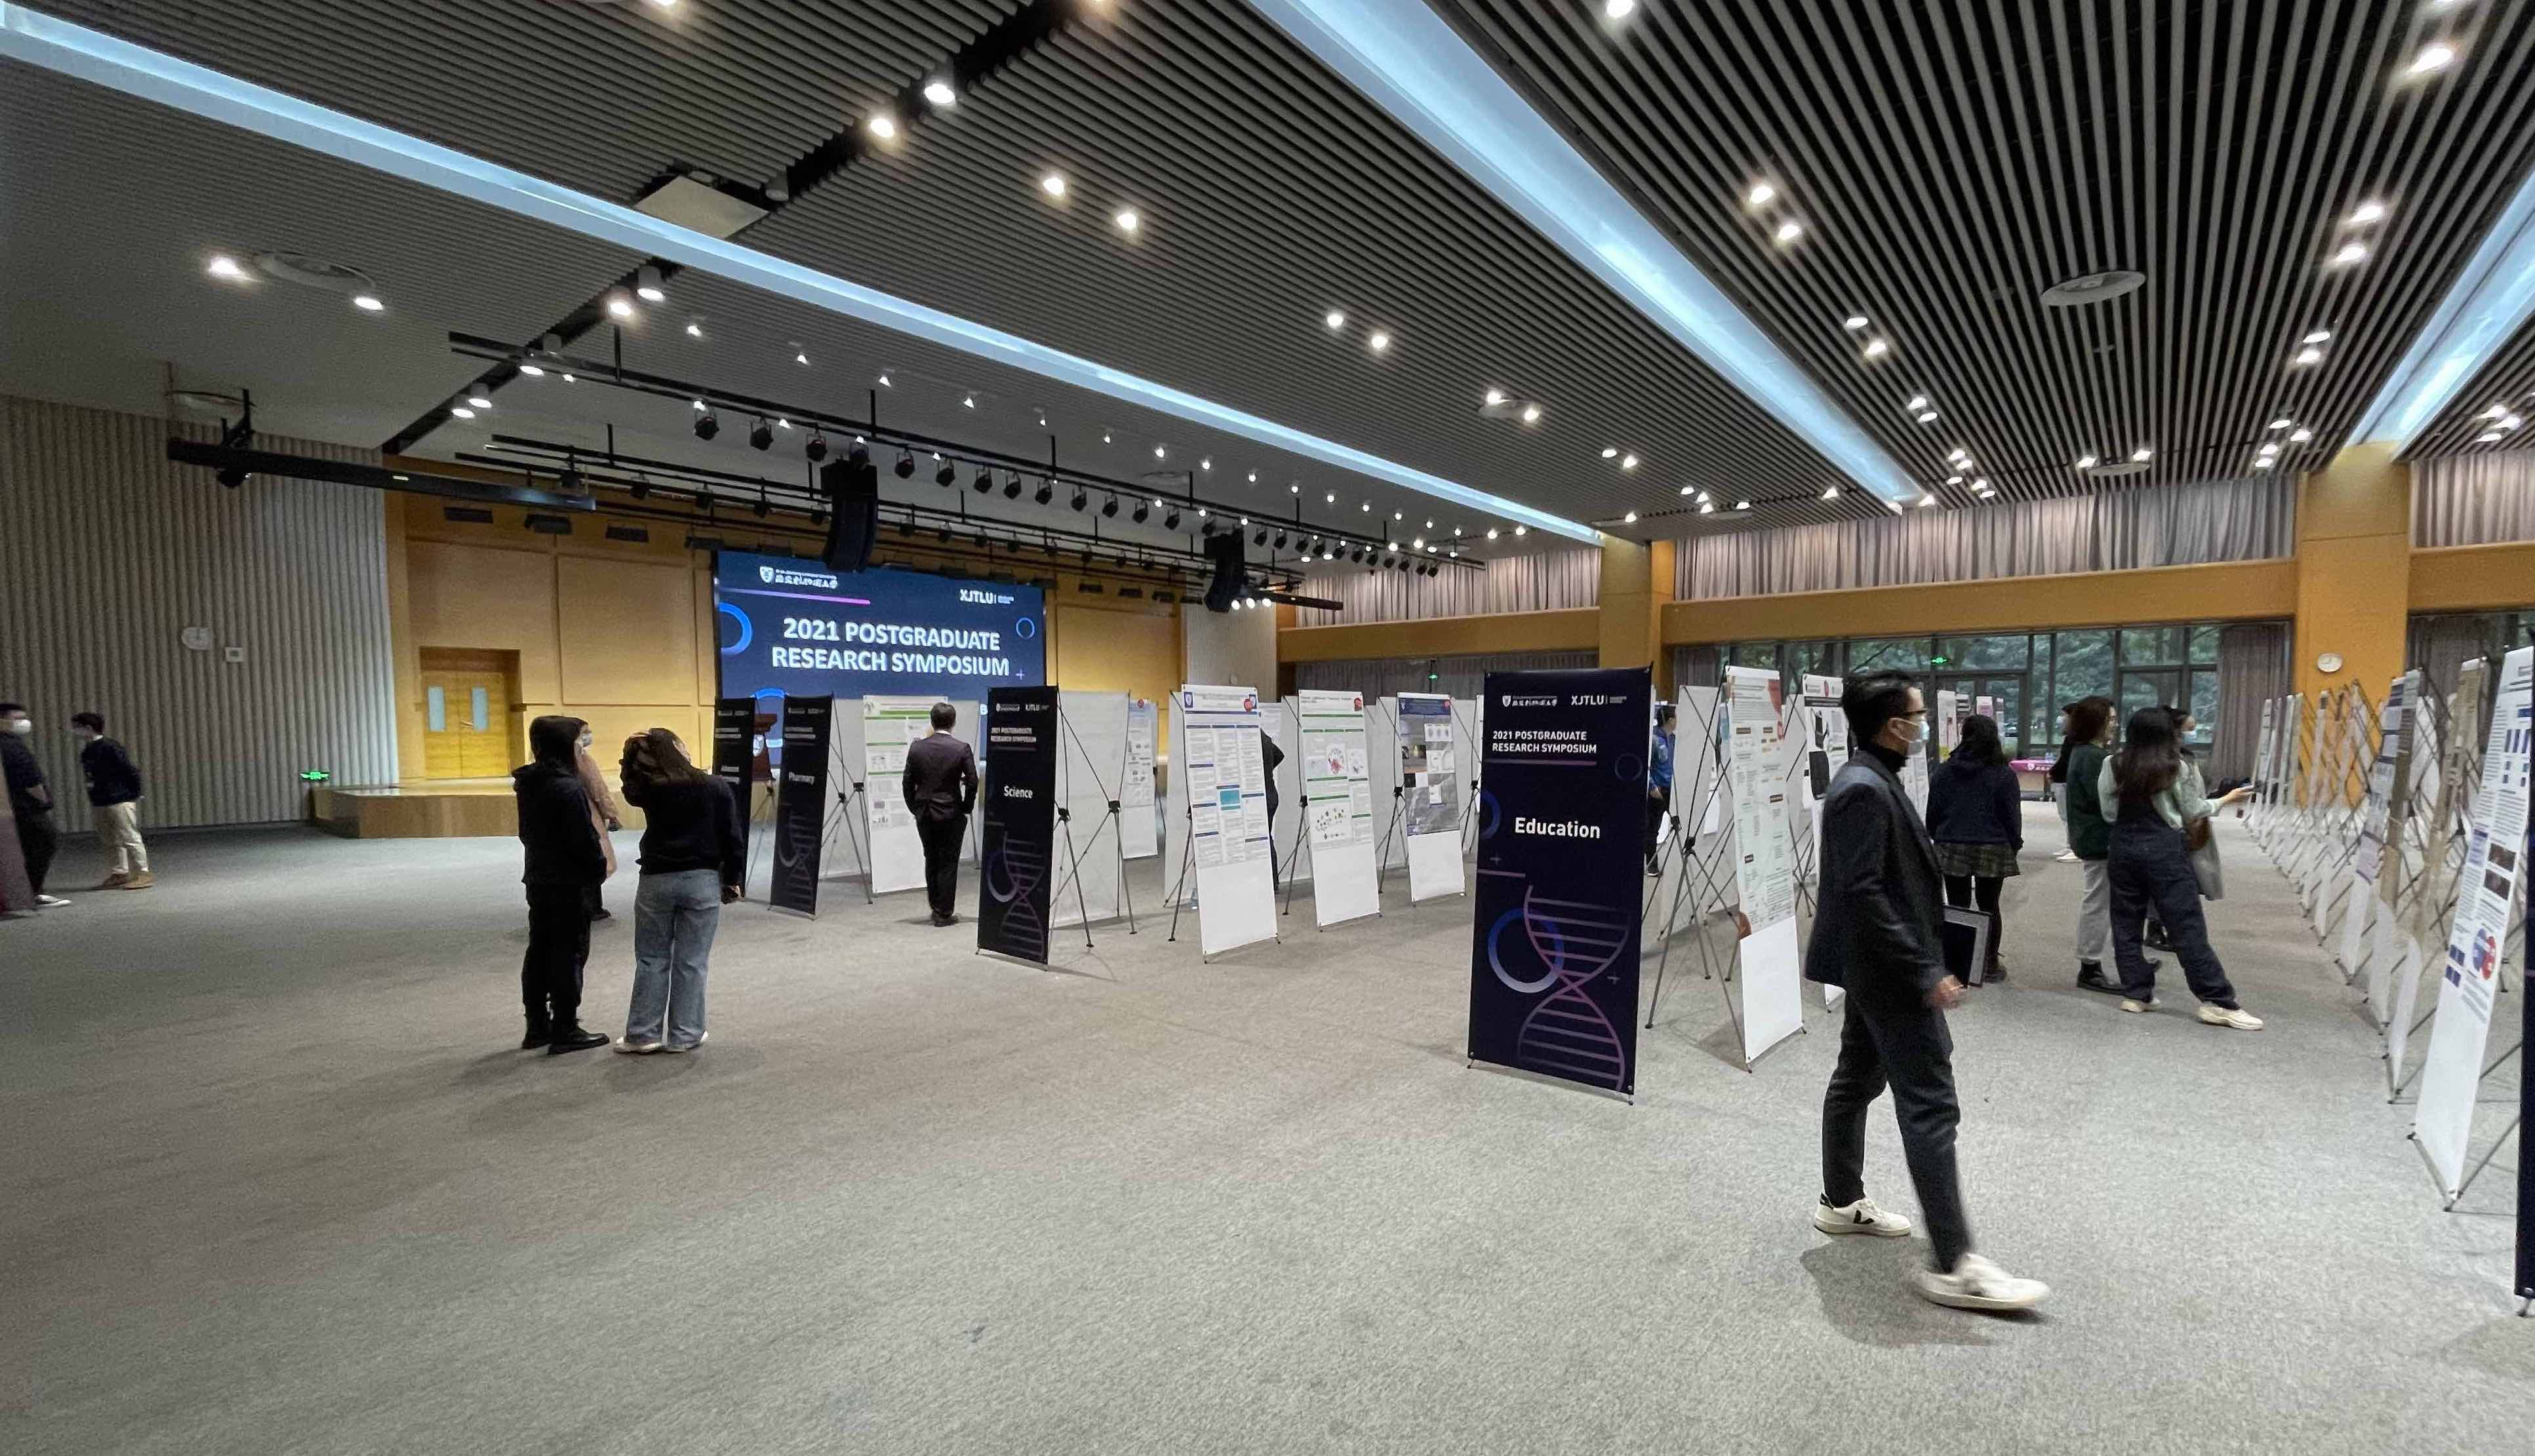
\includegraphics[width=\columnwidth]{author-folder/Kai.Wu/synposium_poster.jpg}
\end{figure}

\subsection{What are the benefits?}

\begin{enumerate}
    \item Improve presentation skills, practice English speaking, and receive guidance from other faculty members
    \item Opportunity to win awards. The university will invite several faculty members to listen to your poster or presentation and score you. Awards include Best Poster Award (10\%), Best Presentation Award (10\%), Excellent Poster Award (20\%), Excellent Presentation Award (20\%), with a certificate and conference funding of 1000 or 500 yuan (for usage of conference funding, see section \ref{sec.fund}). Although it's not a cash reward, it's still useful \sout{(stingy university)}
\end{enumerate}

\begin{figure}[H]
    \centering
    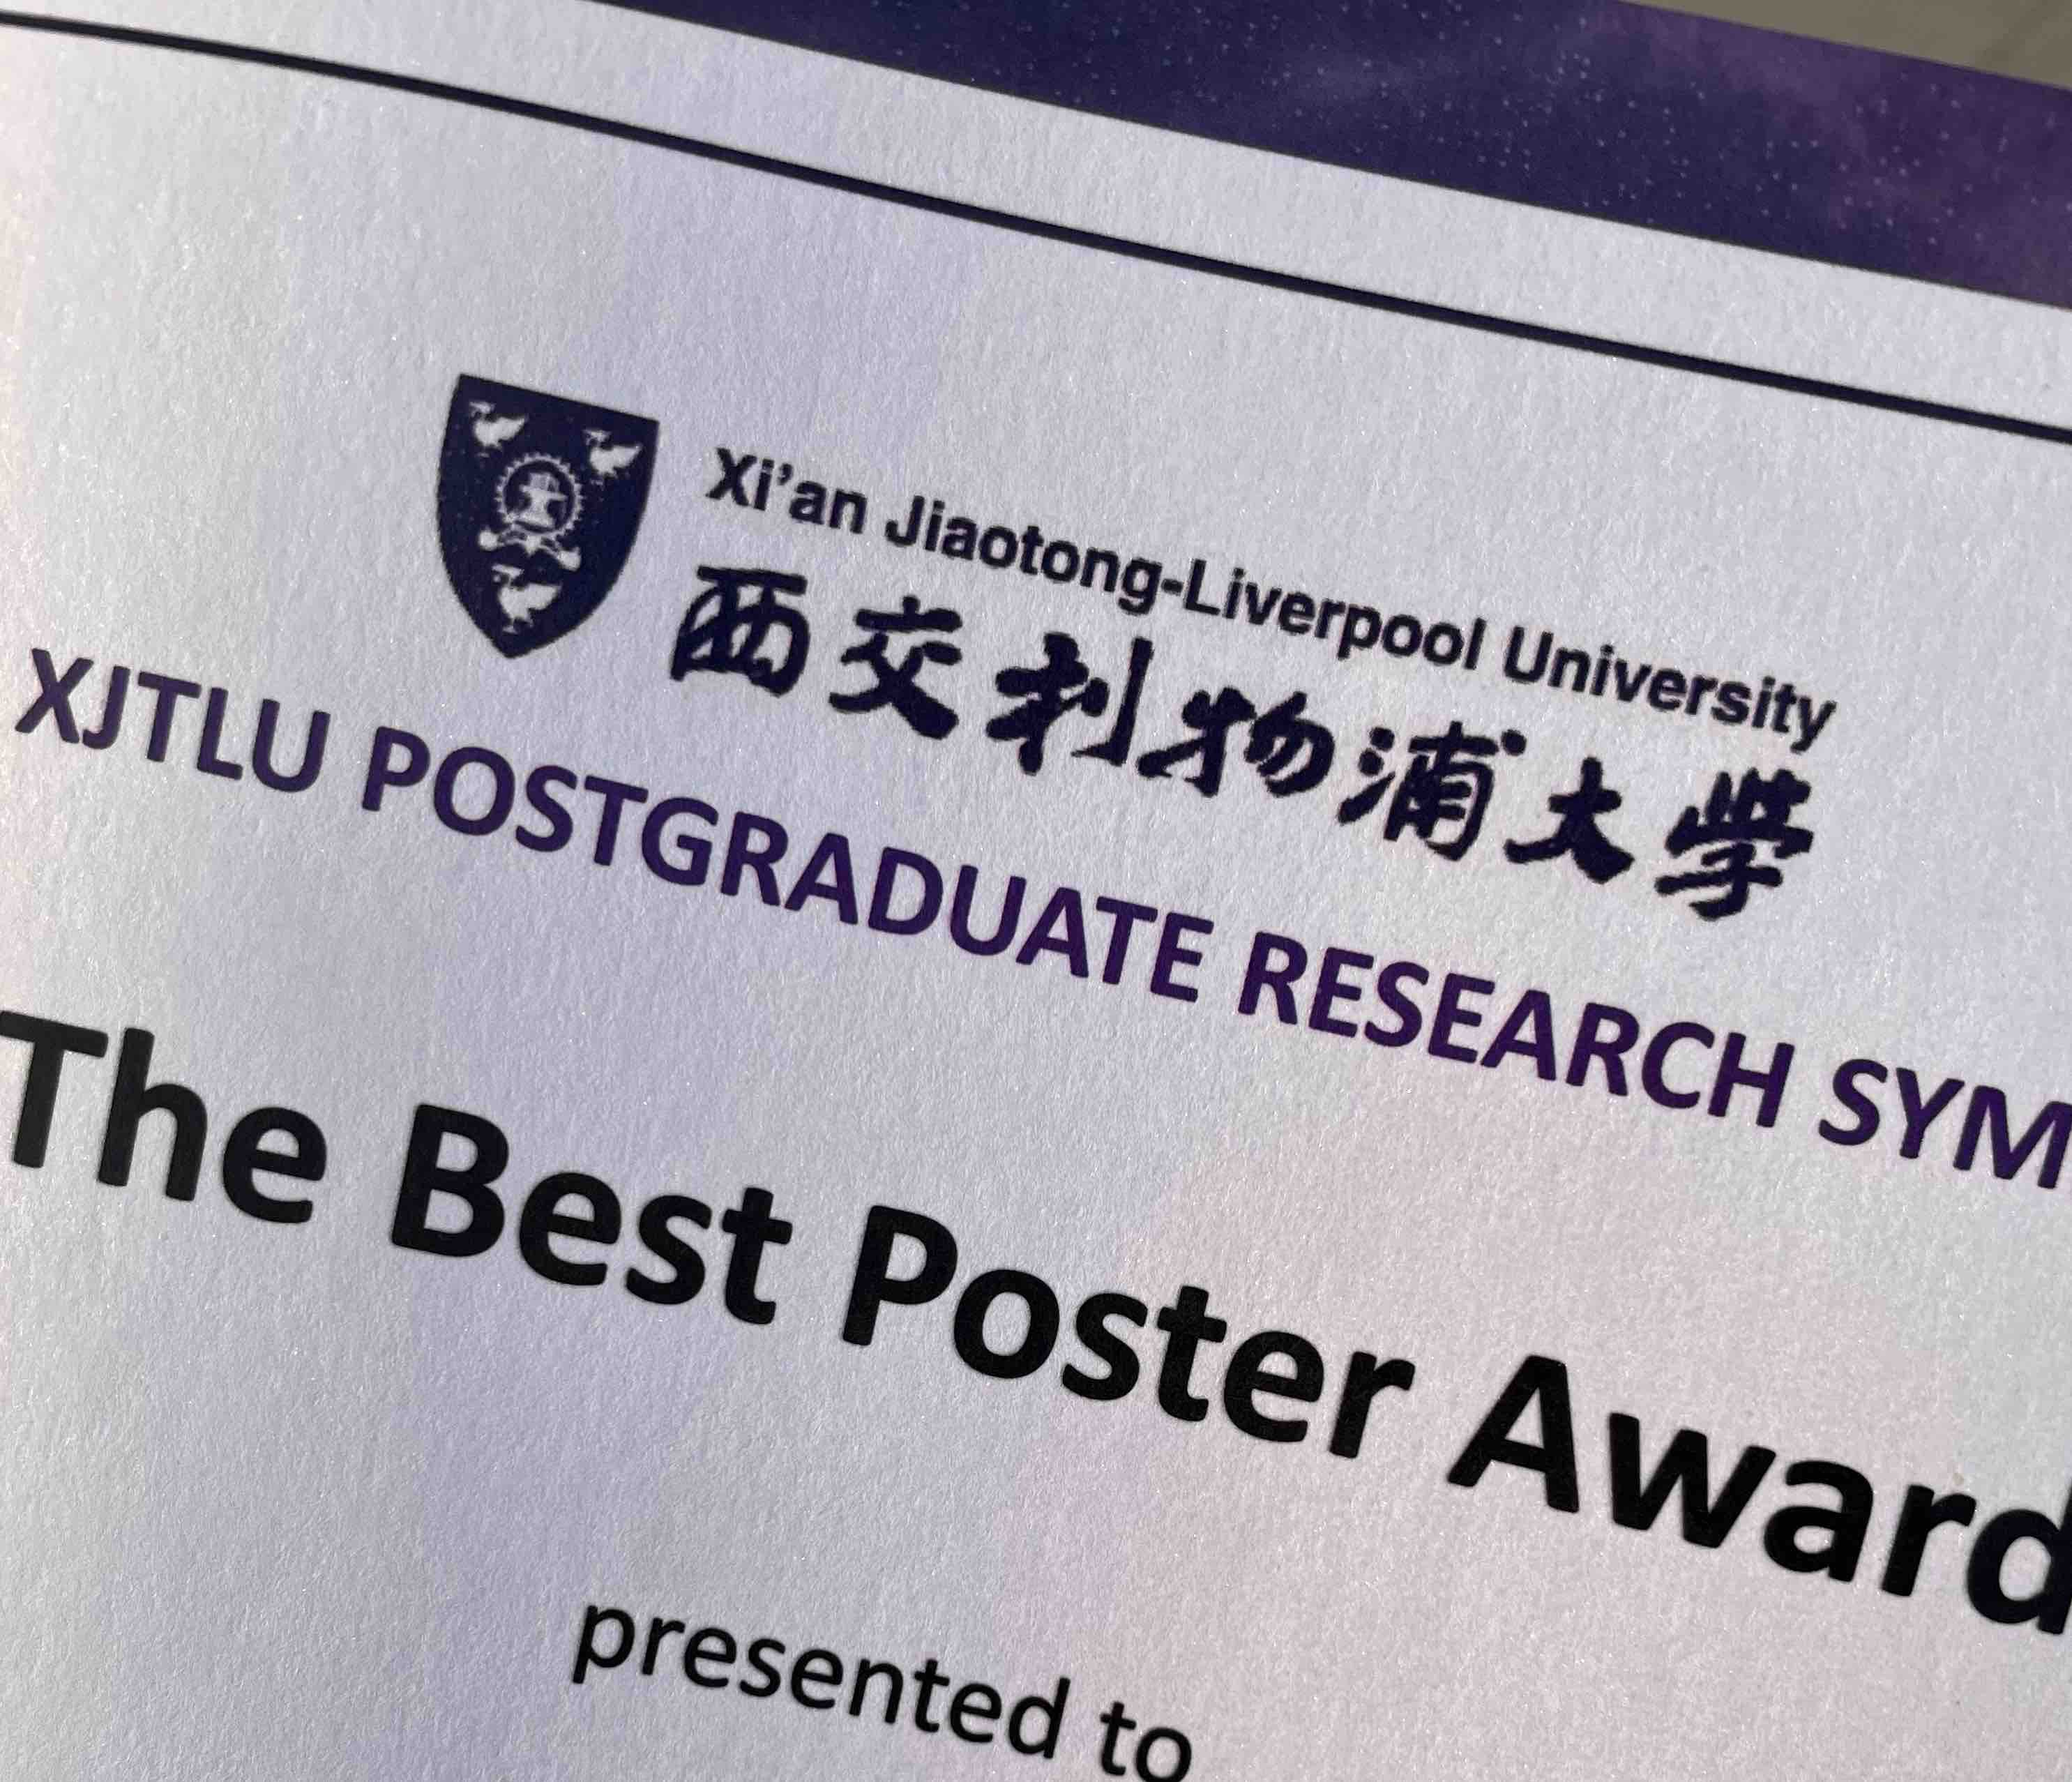
\includegraphics[width=0.4\columnwidth]{author-folder/Kai.Wu/poster_award.jpg}
\end{figure}

\subsection{“I don't want to go”—Try not to!}

Some students often think: the rewards are minimal, the prestige is low, and even winning the best award isn't useful. Moreover, nothing happens if I don't go. Yes, frankly speaking, with your supervisor's consent, you can legally opt out; even if you simply disappear, there likely won't be consequences, and it's unrelated to graduation.

However, as someone who has participated in posters, oral presentations, chaired three oral sessions, and listened to many presentations, unless you are truly adept at giving presentations, I strongly recommend you participate! I've seen students reading scripts with their heads down the entire time, writing scripts directly on their PPTs and reading them, being overly nervous with trembling hands and voices, having PPTs that fail to distinguish primary and secondary points, or being at a loss when facing questions from faculty. Any of these issues would be fatal in your thesis defense!! Remember, our defense isn't a mere formality like at some universities; it's a real challenge where you must deliver a good presentation and answer every sharp question well. \textbf{Do you want to expose these problems during your defense, or discover them early, practice more, and resolve them sooner?}

Therefore, since in the Symposium you won't fail but only be evaluated, and the judges are friendly and will help you identify important issues, \uline{\textbf{it's a very safe and excellent opportunity for practice}}. You shouldn't wait until your defense or attending top conferences to start practicing!

\subsection{Notes and how to perform excellently}

Below is the oral presentation scoring sheet I saw at the 2022 Symposium (can be enlarged for viewing). The considerations for posters are quite similar (participants in the poster session also need to prepare a talk of about 3 minutes to introduce their work to the judges). Frankly speaking, these items are worth noting in any presentation and can be used to carefully review your poster.

\begin{figure}[H]
    \caption{Scoring sheets from 2022}
    \centering
    \begin{tabular}{rl}
        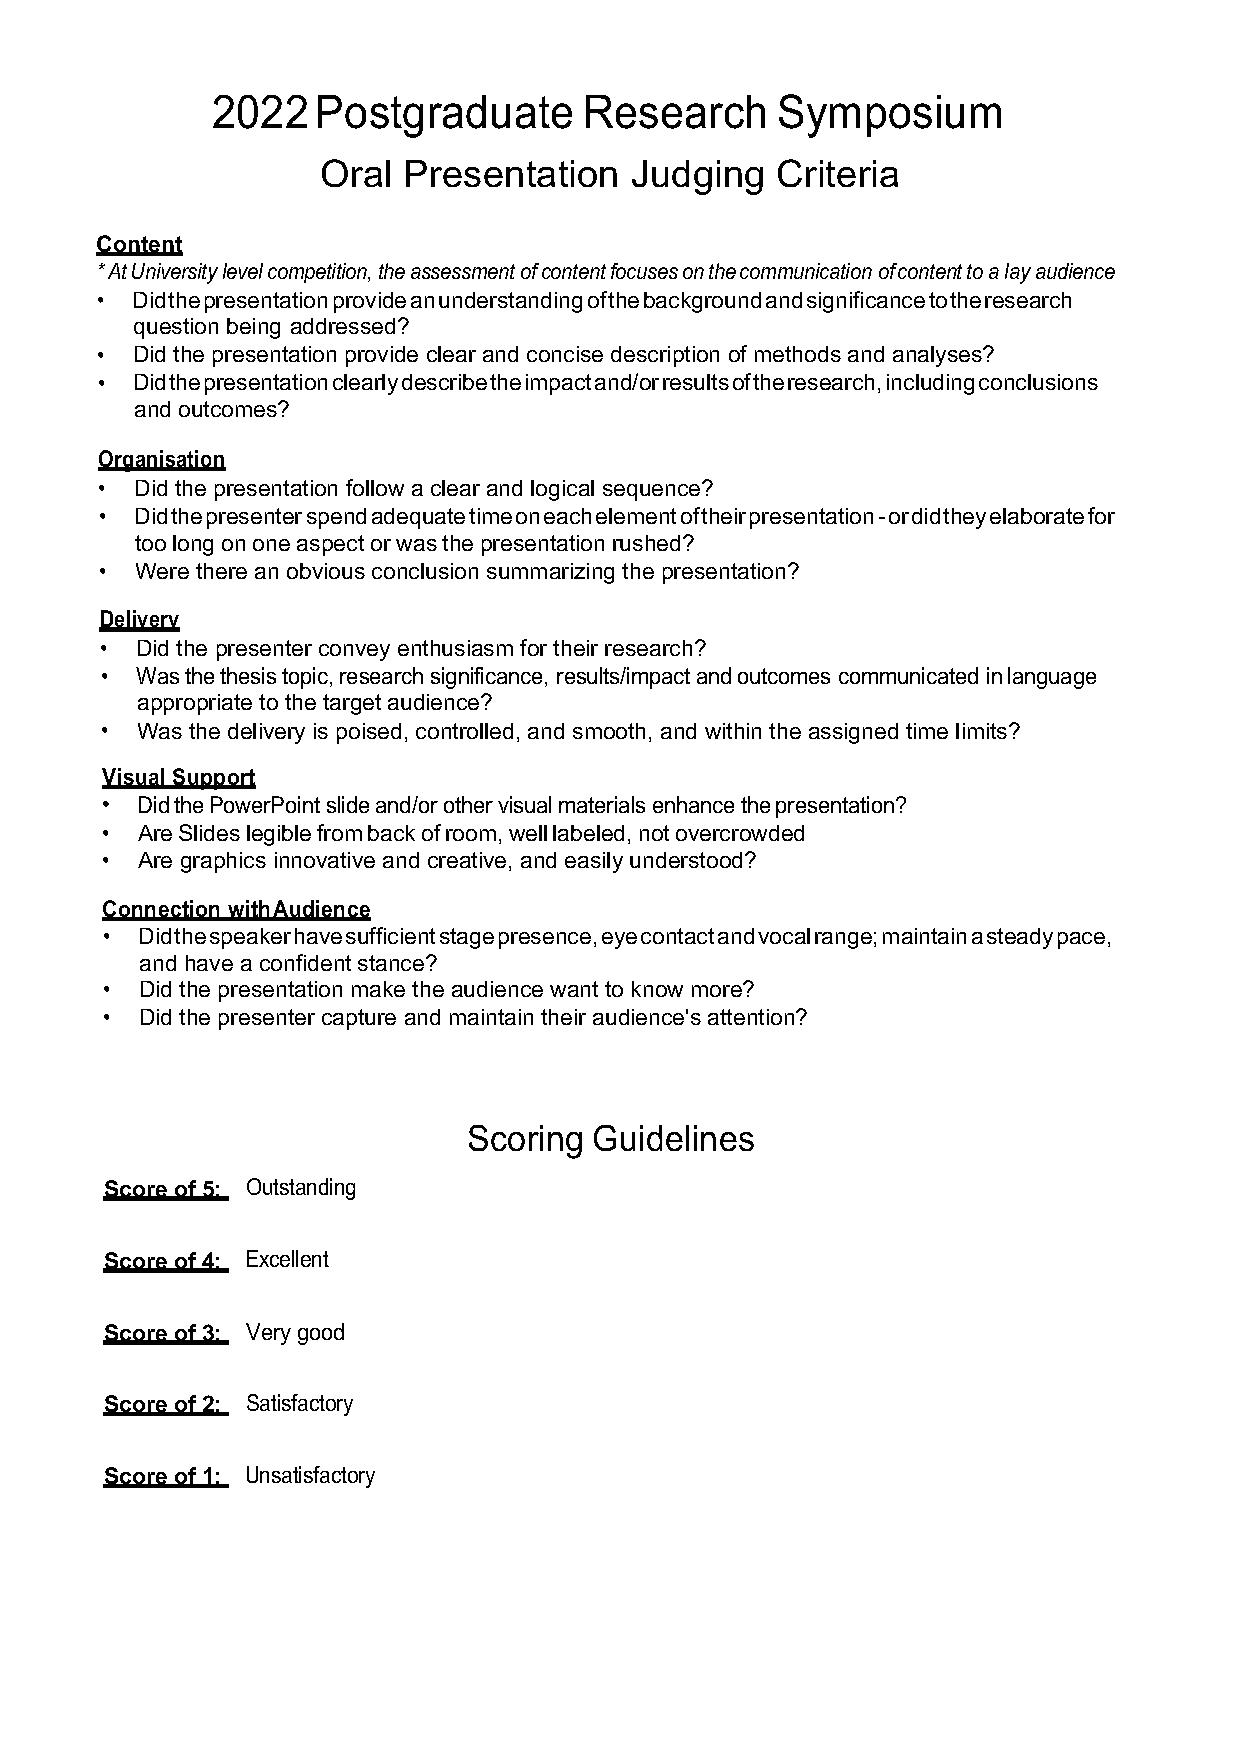
\includegraphics[width=0.5\columnwidth]{author-folder/Kai.Wu/2022_XPGRS_oral_judging_criteria.pdf} & 
        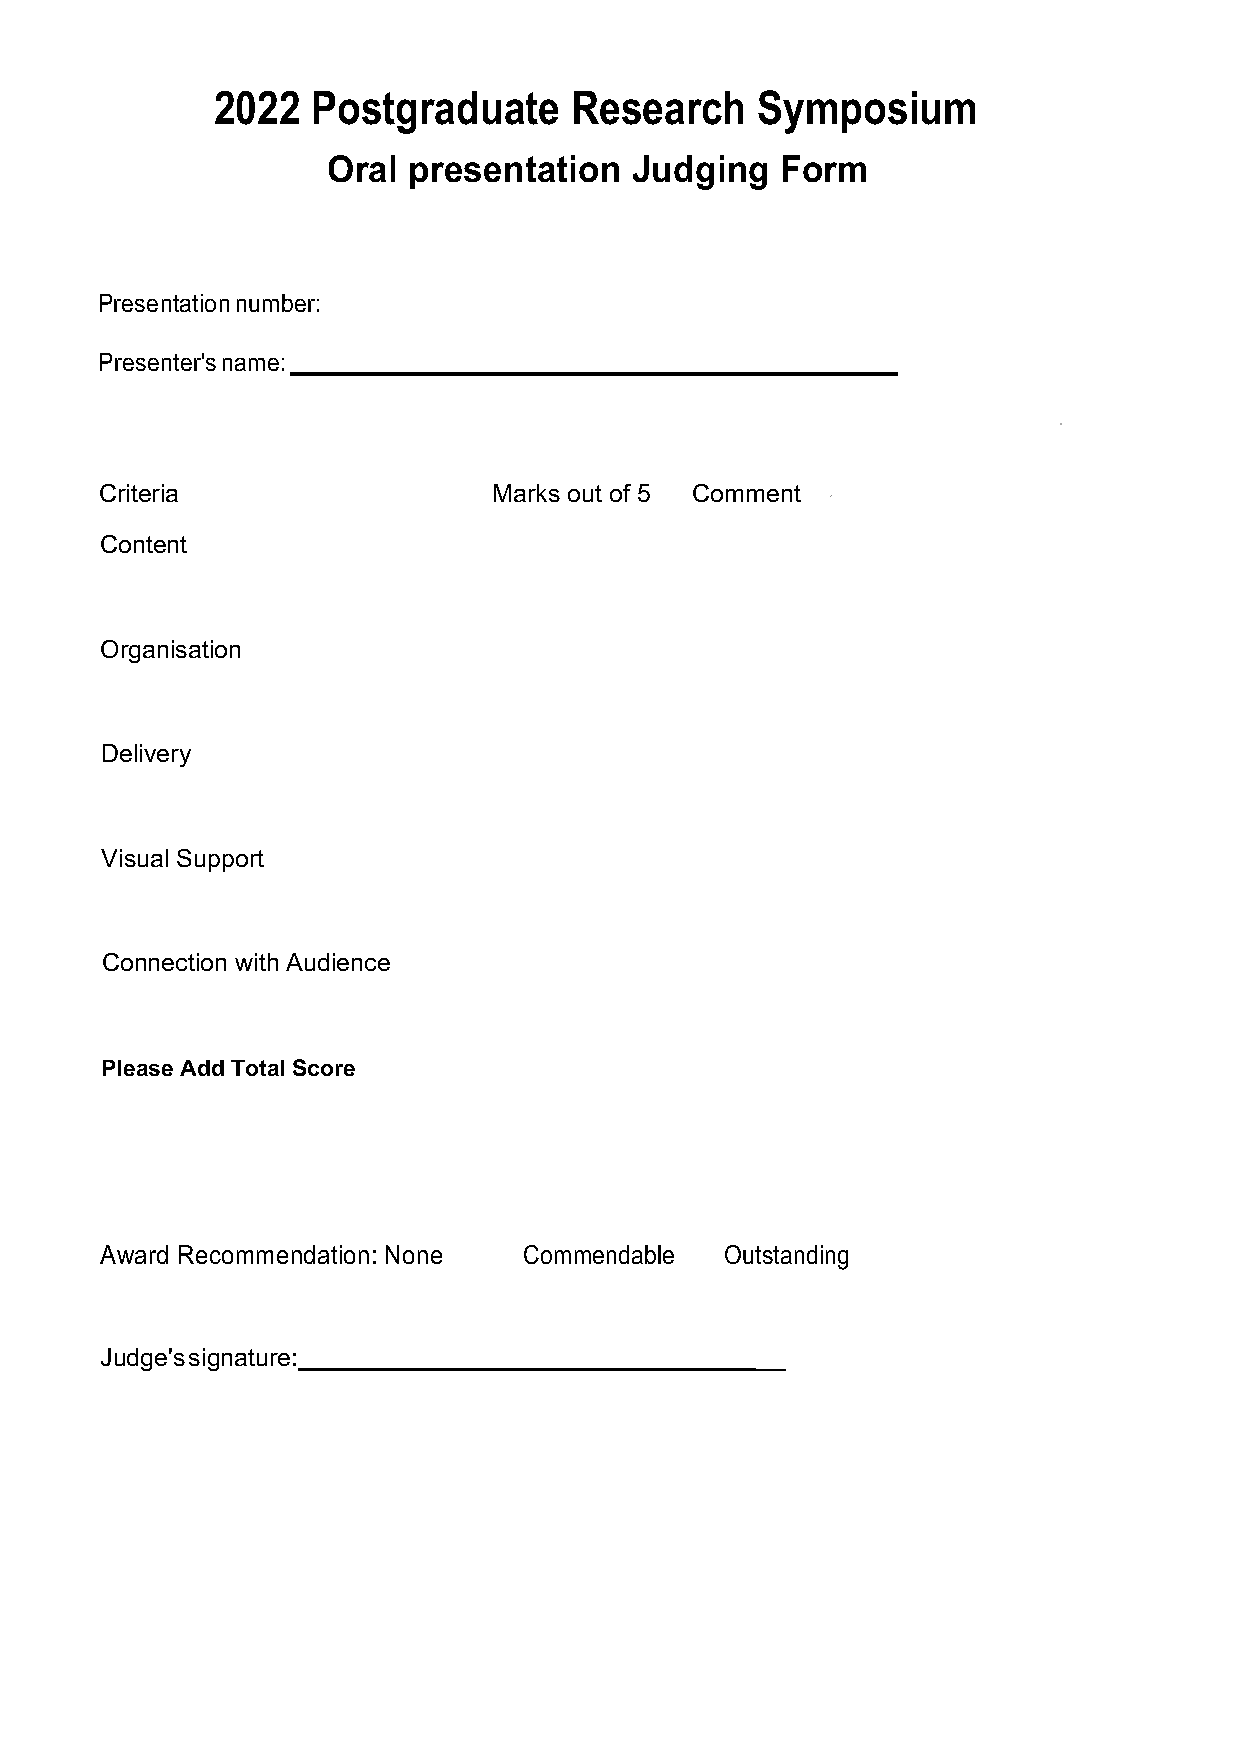
\includegraphics[width=0.5\columnwidth]{author-folder/Kai.Wu/2022_XPGRS_oral_judging_form.pdf} 
    \end{tabular}
\end{figure}

If you want to perform excellently and win awards, you can continue reading below:

There are plenty of tutorials online about giving presentations and making posters. However, the biggest difference between XPGRS and other academic presentations is that the vast majority of students, including the school's judges, may have absolutely no understanding of your research field (as they say, "each profession has its specialty"). If you present as you would to your supervisor, or simply reuse posters or PPTs from academic conferences full of experts, you might not win awards because the judges and other students simply don't understand.

My supervisor told me that XPGRS is different from academic presentations because it's geared toward non-specialists and is more like popular science. Part of the Symposium's goal is to see how you can make non-specialists interested in your research and understand about 70\% of it in a short time. If you're unsure how to do this, imagine one day you meet the Executive President Xi, our  in an elevator—how would you let him know what you're working on, its significance, and ideally pique his interest in a short time? Or, how would you explain your research to relatives or old classmates during the holidays? Academic research isn't done in isolation; being able to present your research and let your academic achievements benefit others is a very important skill.

\begin{flushright}
    October 19, 2022 by \Wu \\
    major update: December 16, 2022 by \Wu \\
    GPT translation proofread by \Shiyao
\end{flushright}